
\documentclass[12pt]{article}
\usepackage{amsmath, amssymb}
\usepackage{array}
\usepackage{booktabs}
\usepackage{geometry}
\usepackage{multirow}
\usepackage{graphicx}
\usepackage{longtable}
\usepackage{float}
\geometry{margin=1in}
\usepackage{tikz}
\usepackage{pgfplots}
\pgfplotsset{compat=1.18} % Use a recent compatibility setting



\begin{document}

    

\begin{center}
    {\LARGE \textbf{Simplified Biostatistics}}\\[6pt]
   Denver JnBaptiste  
\newpage

\tableofcontents

\newpage

\end{center}

\centering \section*{Frequency Distribution}

Frequency distribution helps to quickly see how often each value or group of values appears in your data. It organizes numbers into simple classes so you can easily spot patterns, trends, and make comparisons. This, like all the examples in this book represents a small data set but we use the same logic for a larger dataset. 

\qquad

\centering \textbf{Table 1: Frequency Distribution Table Showing Class Limits and Class Boundaries}

\begin{table}[H]
\centering
\begin{tabular}{c c}
\toprule
\textbf{Class Limits} & \textbf{Class Boundaries} \\
\midrule
30--39 & 29.5--39.5 \\
40--49 & 39.5--49.5 \\
50--59 & 49.5--59.5 \\
60--69 & 59.5--69.5 \\
70--79 & 69.5--79.5 \\
80--89 & 79.5--89.5 \\
90--99 & 89.5--99.5 \\
\bottomrule
\end{tabular}
\end{table}

\noindent
\begin{minipage}[t]{0.48\textwidth}
\centering
\text{Lower boundry}
\vspace{1em}
\begin{align*}
LCB &= LL - \frac{1}{2} \text{ unit of measurement} \\
\\
LCB_1 &= 30 - \frac{1}{2}(1) \\
\\
&= 30 - \frac{1}{2} \\
&= 29\frac{1}{2} \\
\\
&= 29.5 \\
\\
LCB_2 &= 40 - \frac{1}{2}(1) \\
\\
&= 40 - \frac{1}{2} \\
\\
&= 39\frac{1}{2} \\
\\
&= 39.5
\\
\end{align*}
\end{minipage}
\hfill
\begin{minipage}[t]{0.48\textwidth}
\centering
\text{Upper Boundary}
\vspace{1em}
\begin{align*}
UCB &= UL + \frac{1}{2} \text{ unit of measurement} \\
\\
UCB &= 39 + \frac{1}{2}(1) \\
\\
&= 39 + \frac{1}{2} \\
\\
&= 39\frac{1}{2} \\
\\
&= 39.5 \\
\\
LCB_2 &= 49 + \frac{1}{2}(1) \\
\\
&= 49 + \frac{1}{2} \\
\\
&= 49\frac{1}{2} \\
\\
&= 49.5
\end{align*}
\end{minipage}

Class boundaries basically help make sure your data flows smoothly from one class to the next without leaving any gaps. They sit right between the upper limit of one class and the lower limit of the next. This makes the distribution continuous, so every data point has a clear spot to go—no overlaps, no confusion. It keeps histograms accurate and makes statistical work cleaner.

In the examples above, the unit of measurement is 1 (39-40, 49-50... etc. ) and so, we multiply this unit of measurement by 1/2 for the LCB and UCB respectively. You can substitute any unit of measurement based on your class limits to be multiples by 1/2 for class boundaries. For example if the class limits were 35-40 and 45-50, then the unit of measurement would be 5. 

\qquad

We will continue with the same data set above to analyze the class mark. 

\newpage 

\section*{Class Mark}

Class mark is important because it gives the center value of a class. It helps represent the whole class with one number, which makes calculations like mean and graphs easier and quicker.

\[
\text{Class Mark} = \frac{\text{Lower Class Limit} + \text{Upper Class Limit}}{2}
\\
\]

\centering \textbf{Table 2: Class Limits and Class Mark }
\begin{table}[H]
\centering
\begin{tabular}{c c}
\toprule
\textbf{Class Limits} & \textbf{Class Mark} \\
\midrule
30--39 & 34.5 \\
40--49 & 44.5 \\
50--59 & 54.5 \\
60--69 & 64.5 \\
70--79 & 74.5 \\
80--89 & 84.5 \\
90--99 & 94.5 \\
\bottomrule
\end{tabular}
\end{table}

\text{CM}_1 = \frac{30+39}{2}
= 34.5

\\
\text{CM}_2 = \frac{40+49}{2}
= 44.5
etc.

Take a look at the histogram below which represents this data: 

\begin{figure}[H]
    \centering
    \includegraphics[width=0.5\linewidth]{Screen Shot 2025-11-18 at 10.30.01 PM.png}
    \caption{Histogram representing the \textbf{class boundaries} and class \textbf{mark} for data above.}
    \label{fig:placeholder}
\end{figure}

\newpage
\section*{Frequencies}

\textbf{Table 3: Frequency Distribution Table}

\begin{table}[H]
\centering
\begin{tabular}{c c c c}
\toprule
\textbf{Frequency} & \textbf{Relative Freq.} & \textbf{Cumulative Freq.} & \textbf{Relative Cum. Freq.} \\
\midrule
2 & 2/60 & 2 & 2/60 \\
12 & 12/60 & 14 & 14/60 \\
16 & 16/60 & 30 & 30/60 \\
6 & 6/60 & 36 & 36/60 \\
8 & 8/60 & 44 & 44/60 \\
9 & 9/60 & 53 & 53/60 \\
7 & 7/60 & 60 & 60/60 \\
\bottomrule
\end{tabular}
\end{table}

\textbf{The table above shows frequency distribution with Relative Frequencies, Cumulative Frequencies and Relative Cumulative Frequencies. 
}

\qquad

Relative frequency shows how often something happens in proportion to the total. It’s a percentage or decimal of the total.

\qquad

Cumulative Frequency keeps adding up the frequencies as you move down the table. It shows how many values fall up to that point.

\qquad

Relative Cumulative Frequency is the same as cumulative, but in percentage form. It tells you what percent of data falls up to that point.

\newpage

\begin{table}[h!]
    \centering \textbf{Table 4: Frequency Distribution}

\qquad
    
    \begin{tabular}{@{}ccccr@{}}
    \toprule
    \textbf{Class Limits} & \textbf{Frequency ($y$)} & \textbf{Class mark ($x$)} & \textbf{$fx$} \\
    \midrule
    30--39 & 2 & 34.5 & 69 \\
    40--49 & 12 & 44.5 & 534 \\
    50--59 & 16 & 54.5 & 872 \\
    60--69 & 6 & 64.5 & 387 \\
    70--79 & 8 & 74.5 & 596 \\
    80--89 & 9 & 84.5 & 760.5 \\
    90--99 & 7 & 94.5 & 661.5 \\
    \midrule
    \textbf{Total} & \textbf{60} & & \textbf{3880.0} \\
    \bottomrule
    \end{tabular}
\end{table}

The table above demonstrates the values needed to calculate the measures of central tendency (mean, median and mode). 

\newpage

\section*{Mean}

Mean tells you the typical or central value of your data. To find the mean, simply add up all the numbers and divide by the total of the numbers. 

\qquad

We are going to calculate the frequency sample mean of the data presented in our tables so far. 

\qquad


\text{Population mean} \Rightarrow M = \frac{\sum x_i}{\sum f}

\qquad

\text{Sample mean} \Rightarrow \bar{x} = \frac{\sum x_i}{\sum f}

\qquad

\noindent\fbox{%
    \parbox{\textwidth}{%
        \text{Frequency Sample mean} \Rightarrow \bar{x} = \frac{\sum f_i x_i}{\sum f}.
    }%
}

\qquad

$\bar{x} = \frac{\sum f_i x_i}{\sum f}$

\qquad

$\bar{x} = \frac{3880}{60} = 64.67$.

\newpage

\section*{Median}

Median is the middle value when the numbers are arrangeed from smallest to largest. This is especially useful to show the center of data when there are outliers. 

\qquad

If the frequency total of the data is \textbf{odd}, use:
$$\frac{n+1}{2}$$

If frequency total is \textbf{even} use:
$$\frac{\frac{n}{2}+(\frac{n}{2}+1)}{2}$$

After you get the solution to the calculations (odd or even data values), simply look in the \textbf{cumulative frequency} section, for the median cumulative frequency and that would be your solution.

\qquad

For frequency tables where there are class limits, use:
$$L+\left(\frac{\frac{\Sigma f}{2}-B}{G}\right)\times C$$

where \\

\raggedright 

* L = lower class boundary of median group frequency based on cumulative frequency. \\

\qquad

* $\Sigma f$ = frequency total. \\

\qquad

* B = cumulative frequency of group before median group \\

\qquad

* G = frequency of the median group \\

\qquad

* C = group width.

\qquad

\\[2\baselineskip]

\centering

So, the median:

\qquad

Since $\sum f = 60$ (even). $\Rightarrow \frac{n}{2}$

\qquad

$\frac{60}{2} = 30$.

\qquad

So based on the cum freq.

\qquad

$L = 29.5$

\qquad

so median $= 49.5 + \left(\frac{\frac{60}{2} - 14}{16}\right) \times 10$.

\qquad

$= 49.5 + \left(\frac{30 - 14}{16}\right) \times 10$.

\qquad

$= 49.5 + \left(\frac{16}{16}\right) \times 10$.

\qquad

$= 49.5 + 10$.

\qquad

$= 59.5$.

\qquad

So median group is $60-69$.

\qquad


\newpage

\section*{Mode}

\qquad

Mode is the value that appears most often in the data (common or frequent value). 

\qquad

From frequency distributions, the mode can be calculated using the equation below:

\\[2\baselineskip]

Mode: $L + \left(\frac{\Delta_1}{\Delta_1 + \Delta_2}\right) \times C$.

\qquad

$L$ = lower class boundary of number with the most freq.

\qquad

$\Delta_1$ = number in frequency with the most freq before it...

\qquad

$\Delta_2$ = number in freq with 2nd most freq before it...

\qquad

$C$ = distance of limit or boundary/width.

\qquad

\vspace{1em} % Add some vertical space

$\therefore$ Mode $= 49.5 + \left(\frac{(16-12)}{(16-12)+(12-2)}\right) \times 10$

\begin{align*}
&= 49.5 + \left(\frac{4}{4+10}\right) \times 10 \\

\qquad

&= 49.5 + \left(\frac{4}{14}\right) \times 10 \\

\qquad

\displaystyle{\displaylines{&= 49.5 + \frac{20}{7} \\}}

\qquad

&= 52.357

\qquad

\end{align*}


\newpage

\section*{Sum of Squares}

\qquad

Sum of squares is the total of all squared differences from the mean. This can show how spread out the data is. \textbf{So, the bigger the sum of squares, the more spread out your data }

\qquad

The sum of squares is actually the base for some other statistical outlooks such as variance, standard deviation, ANOVA, regression principle component analysis and more. 

\qquad

The equation for sum of squares is seen below: 


$$SS = \Sigma fx^2 - \frac{(\Sigma fx)^2}{\Sigma f}$$

\vspace{1cm}

\centering \textbf{Table 5: Frequency Distribution with $x^2,  fx^2$ values}

\qquad

\begin{tabular}{ccccc}
\toprule
Class mark ($x$) & frequency ($f$) & $x^2 & fx^2$ & $fx$ \\
\midrule
34.5 & 2 & 1190.25 & 2380.5 & 69 \\
44.5 & 12 & 1980.25 & 23763 & 534 \\
54.5 & 16 & 2970.25 & 47524 & 872 \\
64.5 & 6 & 4160.25 & 249615 & 387 \\
74.5 & 8 & 5550.25 & 44402 & 596\\
84.5 & 9 & 7140.25 & 64262.25 & 760.5 \\
94.5 & 7 & 8930.25 & 62511.75 & 661.5 \\
\midrule
Total & 60 & & 269805 & 3880 \\
\bottomrule
\end{tabular}

Table showing the set up for sum of squares calculations.

\vspace{1cm}

$$SS = 269805 - \frac{(3880)^2}{60}$$

\qquad

$$= 269805 - \frac{15054400}{60}$$

\qquad

$$= 269805 - 250906.67$$

\qquad

$$= 18898.33$$

\newpage

\section*{Variance:}

\qquad

Variance shows how spread out the data is from the average (how many data points vary or deviate from the center). 

\qquad

So: If all values are close to the mean → low variance (data is consistent).

If values are far from the mean → high variance (data is spread out).

\subsection*{Sample variance (subset of population):}

$$S^{2} = \frac{\sum f(x)^{2} - \frac{(\sum fx)^{2}}{\sum f}}{\sum f - 1}$$

notice sample variance $\Rightarrow \frac{SS}{\sum f-1}$

\subsection*{Population variance:}

$$\sigma^{2} = \frac{\sum(x_{i}-\mu)^{2}}{N}$$

so, in our problem:

\qquad

Sample variance $= \frac{18898.33}{60-1}$

\qquad

$S^{2} = 320.31$

\qquad

Population variance = $\sigma^{2}=\frac{\sum(x_{i}-\mu)^{2}}{n}

\qquad

$=(34.5-64.67)^{2}+(44.5-64.67)^{2}+(54.5-64.67)^{2}+$
$(64.5-64.67)^{2}+(74.5-64.67)^{2}+(84.5-64.67)^{2}$
$+(94.5-64.67)^{2}$
60

\newpage

\section*{Standard deviation}

\qquad

Standard deviation is a measure that shows how spread out the values in a dataset are from the mean (average).

\qquad


If the standard deviation is small → the data points are close to the mean (less variation).

\qquad

If the standard deviation is large → the data points are far from the mean (more variation).

\\[2\baselineskip]

The formula for standard deviation is below: 

\qquad

$S = \sqrt{S^2} \Rightarrow \text{Sample standard deviation}$

\qquad

Below is how we calculate standard deviation:

\qquad

$\sigma = \sqrt{\sigma^2} \Rightarrow \text{Population standard deviation}$

$\therefore \text{Since } S^2 = 320.31$

$S = \sqrt{320.31}$

$= 17.9$

Coefficient of variation $\Rightarrow V$

\qquad

$V = \frac{S}{\bar{x}} \times 100 \%$

\qquad

$\therefore V = \frac{17.9}{64.67} \times 100$

\qquad

$= 0.277 \times 100$

\qquad

$= 27.7 \%$

\newpage

\section*{Binomial Distribution}

\qquad

Binomial distribution is used when you’re counting how many times something succeeds out of a fixed number of trials, where:

\qquad

\raggedright

* Each trial has two outcomes, this deals with success or failure, head/tail, pass/fail etc.

\qquad

* The number of trials (n) is fixed.

\qquad

* The probability of success (p) stays the same each time.

* All trials are independent, one outcome doesn't affect the next.

\vspace{1cm}

\centering

\begin{tabular}{|l|c|}

\hline
Class limits & Frequency \\
\hline
30-39 & 2 \\
40-49 & 12 \\
50-59 & 16 \\
60-69 & 6 \\
70-79 & 8 \\
80-89 & 9 \\
90-99 & 7 \\
\hline
Total & 60 \\
\hline
\end{tabular}
\hfill

\vspace{1cm}

If we are dealing with success or failure: 

\qquad

A) $P(x \ge 60) = \frac{6+8+9+7}{60} = \frac{30}{60} = 0.5$

\qquad

B) What if, out of our data, a sample of 6 students was selected; what is the probability of all 6 scoring below 60.

\qquad

Since $P(x \ge 60) = 0.5$, then $P(x < 60) = 1 - 0.5 = 0.5$.

\qquad

Therefore, the probability of all 6 scoring below 60 is $P^6 = (0.5)^6 = 0.016$.

\qquad

c) The probability of the first 4 Scarfing 60 or more.

$$\binom{6}{4} (p^4 q^2) = \binom{6}{4} (0.5)^4 (0.5)^2$$
$$= 15(0.0156)$$
$$= 0.234$$

Other useful formulas for Binomial Distribution:

\qquad

mean $\Rightarrow \bar{x} = np$
variance $\Rightarrow s^2 = npq$
Standard deviation $\Rightarrow s = \sqrt{npq}$

\newpage

\section*{Poisson Distribution}

Poisson Poisson distribution shows many times an event is likely to happen in a fixed time or space, when:

\qquad

\raggedright

* The event happens randomly.

\qquad

* It happens independently (one does not affect another).

\qquad

* It happens at an average known rate lambda (λ).

$$P(x)=\frac{\mu^{x}}{e^{u}x!}$$

\centering

\qquad

where $\mu$ is the Parameter of the distribution.

\qquad

Poisson distribution approaches the binomial distribution where $n$ is large and $p$ is very small.

\qquad

$\sigma^2$ in poisson distribution also $= \mu$; in Binomial they are different.

\qquad

Poisson can be used if $p$ is very small, $N$ is $\ge 30$.

\qquad

If $N$ is small, Binomial is used.

\qquad

eg. If there are 90 cars and $2\%$ normally have defective bolts. What is the probability that 6 bolts are found defective?

\qquad

Sol: $n=90$

\qquad

$2\%=0.02$.

\qquad

So: $m=(90)(0.02)$
$= 1.8$

\qquad

So: $P(x) = \frac{u^x}{e^u x!} = \frac{1.8^6}{e^{1.8}(6!)} = \frac{1.8^6}{4.355.7} = 0.0078...$

\qquad

P(X<2) \text{ are defective: } = P(X=1)+P(X=0)
$$
=\frac{1.8^{1}}{e^{1.8}(1!)}+\frac{1.8^{0}}{e^{1.8}(0!)}
$$
$$
= 0.298 + 0.165
$$
$$
= 0.463
$$
$P(X\ge 2)=1-\{P(X<2)\}$
$$
= 1-0.463
$$
$$
= 0.537
$$
Coefficient of dispersion is found when Poisson is concerned, it checks for randomness for Poisson because u a variance = 1.
$$
CD=\frac{s^{2}}{\overline{x}}.
$$

\newpage

\section*{Normal Distribution}

Normal distribution is \textbf{symmetric around the mean,} where most values cluster near the mean and fewer values occur as you move farther away.

\begin{itemize}
    \item mean = median = mode
    \item random \& independent
    \item expected value = mean
    \item variance = 1, standard deviation = 1
    \item standard score/deviate = Z-score
\end{itemize}

\begin{figure}[h!]
    \centering
    \includegraphics[width=0.5\linewidth]{Screen Shot 2025-11-20 at 8.24.15 PM.png}
    \textbf{\caption{Bell Shaped Probability Distribution- Normal Distribution}}
\end{figure}

$$Z = \frac{x_i - \mu}{\sigma}$$

If $\mu = 64.67$ mm and we are asked what proportion of the population is greater than 67 mm.

$$Z = \frac{67 - 64.67}{17.9}$$

$$= 0.130$$

So: $P(x_i > 67\text{mm}) = P(Z > 0.13) = 0.5517$. from the normal distribution table.

two tailed = 0.5517. \\

\qquad

one tailed = 0.4483 \\

\qquad

So: $1 - 0.4483$ \\

\qquad

$= 0.5517$ \\

\begin{figure}[h!]
    \centering
    \includegraphics[width=0.5\linewidth]{image.png}
    \caption{Two tailed distribution}
\end{figure}

\newpage

\section*{Confidence Intervals}

\qquad

Confidence intervals are range values, calculated from sample data. 
CI's show how sure we about an estimate made. CI's are normally represented as percentages (95% CI). 

\qquad

\raggedright

1) $P\left(-t_{\alpha/2, v} \le \frac{\bar{x} - \mu}{s_{\bar{x}}} \le t_{\alpha/2, v}\right) \quad 1-\alpha$

\qquad

2) $P\left(-Z \le \frac{\bar{x} - \mu}{\sigma_{\bar{x}}} \le Z\right)$

\qquad

3) $\frac{vs^2}{\chi^2_{\alpha/2, v}} \le \sigma^2 \le \frac{vs^2}{\chi^2_{1-\alpha/2, v}}$

\newpage

\centering

\section*{Confidence Limits}

\qquad

Confidence limits are lower and upper boundaries of CI's

$L_{1} = \bar{x} - z\sigma_{\bar{x}}$ 

\qquad

$L_{2} = \bar{x} + z\sigma_{\bar{x}}$

\qquad

for $Z$, the same principle of upper and lower limits can be applied for $t$ \& $\chi^2$ (chi square).

\section*{Test Statistics}

\qquad

Test statistics are numbers calculated from sample data that are used to decide whether to reject or accept a null hypothesis in a statistical test.

\qquad

Test statistics should not be confused with statistics tests as we have been doing. Test statistics summarize the difference between what you observe in your data and what you would expect under the null hypothesis, often in terms of standard errors.

\qquad

Examples of test statistics include t, z, chi-square, and F values.

\qquad

\begin{enumerate}
    \item $t = \frac{\bar{x} - \mu}{s_{\bar{x}}}$ \quad if $\sigma$ is unknown, $n < 30$
    \item $Z = \frac{\bar{x} - \mu}{\sigma_{\bar{x}}}$ \quad if $\sigma$ is known, $n \ge 30$
    \item $\chi^2 = \frac{s^2v}{\sigma^2}$ Skewed to the right (chi square).
\end{enumerate}

\qquad

The null is accepted if there is no significant difference between the observed and the expected. If the null is rejected, the alternative is true and there is significant difference between the observed and the expected. 

\newpage

\section*{Analysis of Variance (Anova)}

\qquad

Anova compares the means of three or more groups to see if at least one group mean is significantly different from the other group means.

It works by analyzing the variance within groups versus the variance between groups.

\subsection*{One way Anova:}
\begin{enumerate}
    \item Fixed
    \item Random
\end{enumerate}
*fixed = specific levels of interest, random = sampled from a larger population

\qquad

$\implies$ 1 null hypothesis is needed for one way Anova

\subsection*{Two way Anova:}
\begin{enumerate}
    \item without replication (2 null hypotheses)
    \item with replication (3 null hypotheses)
\end{enumerate}

One Way Anova determines whether there is any statistical significance between means of three or more groups that are not related.

So $H_{0} = \mu_{1} = \mu_{2} = \mu_{3} \dots \mu_{k}$

\begin{table}[h]
    \centering
    \begin{tabular}{|c|c|c|c|}
        \hline
        Cars & X & Y & Z \\
        \hline
        & 8 & 6 & 8 \\
        & 9 & 2 & 9 \\
        & 5 & 3 & 7 \\
        & 3 & 4 & 5 \\
        \hline
        Total & 25 & 15 & 29 \\
        \hline
    \end{tabular}
\end{table}

$\text{mean} = x 6.25 \quad y3.75 \quad z7.25$

$\text{SD} = x2.75 \quad y1.71 \quad z1.71$

$\text{Grand total} = 69$

\begin{table}[h]
    \centering

    \begin{tabular}{|l|c|c|c|c|c|}
        \hline
        Source of variance & SS & df & MS & $\text{F}_{S}$ & $\text{F}_{\text{table}}$ \\
        \hline
        Among cars & 26 & 2 & 13 & 2.91 & $\text{F}_{0.05}(2,9)$ \\
        within cars & 40.25 & 9 & 4.47 & & $= 4.26$ \\
        \hline
        Total cars. & 66.25 & 11 & & & \\
        \hline
    \end{tabular}
\end{table}

from the "F" table for test statistics: If $\text{F}_{S} > \text{F}_{\text{table}}$ reject.

\qquad

\begin{align*}
\text{SS among} &= \frac{(\sum A)^2}{n} - \frac{(\text{Grand total})^2}{N} \\
&= \frac{2S^2 + 1S^2 + 2q^2}{4} - \frac{(6q)^2}{12} \\

\displaystyle{\displaylines{&= \frac{1691}{4} - \frac{4761}{12} \\}}

\qquad

&= 563.67 - 396.75 \\

\qquad

&= 26.
\end{align*}
\begin{align*}
\text{Total SS} &= \sum A^2 - \frac{(\text{Grand total})^2}{N} \\
&= \left( (8^2 + 9^2 + 5^2 + 3^2) + (6^2 + 2^2 + 3^2 + 4^2) + (8^2 + 9^2 + 2^2 + 5^2) \right) - 396.75 \\
&= 463 - 396.75 \\
&= 66.25
\end{align*}

\begin{align*}
\text{Within SS} &= \text{Total SS} - \text{Among SS} \\
&= 66.25 - 26 \\
&= 40.25
\end{align*}

\newpage

\section*{Multiple Comparison test as part of Anova}

\qquad

The Multiple Comparison Test (also called post-hoc test) is done after ANOVA if you find a significant difference, this helps determine which specific group means are different from each other.

\qquad

Common methods include:

\raggedright

* Tukey’s HSD (Honestly Significant Difference) – controls overall error rate

\qquad

* Bonferroni – adjusts for multiple comparisons

\qquad

* Scheffé – more conservative

\qquad

So, ANOVA tells you there is a difference somewhere in the represented data; multiple comparison tests tell you exactly where you can find that difference.

\qquad

\centering

\textbf{Least Significant Difference (LSD)}

\qquad

The Least Significant Difference (LSD) is a type of multiple comparison (post-hoc) test.

\qquad

It compares pairwise differences between group means.

\qquad

If the difference between two means is greater than the LSD value, it’s considered statistically significant.

\qquad

LSD has a higher chance of \textbf{Type I error} (reject the null hypothesis even though it is actually true - you think there is an effect when there is actually no effect) when many comparisons are made because it is not very conservative. 

\qquad

*Since we are on this topic or errors: False Negatives are type two errors: Failing to reject the null hypothesis when it is false.

\qquad

BACK TO LSD:

$$ \text{LSD} = t_{\alpha(\text{df})} \sqrt{MS_w \left(\frac{1}{n_1} + \frac{1}{n_2}\right)} $$

Control vs y

\qquad

Control vs x

\qquad

Control vs z

\qquad

means:
Control = 6,
y = 3.75,
x = 6.25,
z= 7.25     

Since x, y, \& z has the same n(4) we can use the same LSD for each comparison.

$$ \text{LSD} = t_{0.05(9)} \sqrt{4.47 \left(\frac{1}{4} + \frac{1}{4}\right)} $$

$$ = 2.262 \sqrt{4.47 \left(\frac{2}{4}\right)} $$

$$ = 2.262 (1.49) $$

$$ = 3.37 $$

For control vs y:
$$ |6 - 3.75| = 2.25 $$

$$ 2.25 < \text{LSD} $$

Therefore, accept $H_0$.

\newpage

\section*{Student - Newman - Keul (SNK) Comparison}

\qquad

This is another post-hoc test, used after ANOVA and helps identify which group means are significantly different.

\qquad

It orders group means from smallest to largest.

\qquad

Compares all pairs stepwise, starting with the largest difference.

\qquad

Less conservative than Tukey’s HSD, so it has a higher chance of Type I error.

\qquad

Useful when you want more power to detect differences but accept slightly higher error risk.

Helps find which group means differ after ANOVA

\qquad

\begin{tabular}{l|l|l|l|l|l|l}
\toprule
Comparison & Difference & SE & P-range & $q = \frac{\text{Diff}}{\text{SE}}$ & $Q(2, 9)$ (from table) & Decision \\
\midrule
x vs y & $6.25 - 3.75$ & $\frac{\sqrt{ms_w}}{\sqrt{n}}$ & 2 & $\frac{2.5}{1.06}$ & 3.199 & accept $H_0$ \\
& $= 2.5$ & $= \sqrt{\frac{4.47}{4}}$ & & $= 2.36$ & & \\
& & $= 1.06$ & & & & \\
\bottomrule
\end{tabular}

\newpage

\section*{Independent T-test}

\qquad

The data for independent T-tests is assumed to be normally distributed and has similar variances

The Independent T-test is also called two-sample t-test. It is used to  compare the means of two independent groups to see if they are significantly different.

\qquad

\vspace{0.5cm}

\begin{tabular}{lcc}
\textbf{Boys} & \textbf{Girls} & \\
8 & 5 & \\
3 & 4 & \\
2 & 3 & \\
8 & 2 & \\
9 & 8 & \\
10 & 10 \\
\hline
40 & 32 \\

\end{tabular}

\qquad

Formula: 

\qquad

$t_{s} = \frac{\bar{x}_{1} - \bar{x}_{2}}{\sqrt{\frac{s_{1}^{2}}{n_{1}} + \frac{s_{2}^{2}}{n_{2}}}}$

\vspace{0.5cm}

$\bar{x}_{1} = \frac{40}{6} = 6.67$

\qquad

$s_{1}^{2} = 11.07$

\qquad

$\bar{x}_{2} = \frac{32}{6} = 5.33$

\qquad

$s_{2}^{2} = 9.47$

\vspace{0.5cm}

So: $t_{s} = \frac{6.67 - 5.33}{\sqrt{\frac{11.07}{6} + \frac{9.47}{6}}}$

\qquad

$= \frac{1.34}{\sqrt{3.42}}$

\qquad

$= 0.72$

\vspace{0.5cm}

$t_{0.05((n_{1}+n_{2})-2)}$

\qquad

$t_{0.05(10)} = 2.228$

\qquad

So $t_{s} < t_{\text{table}} \Rightarrow \text{accept } H_{0}$.

\newpage

\section*{Two-way Anova with replication}

\qquad

Recall: Anova compares the means of three or more groups to see if at least one group mean is
significantly different from the other group means.

\qquad

Two way Anova examines the effect of two independent factors on a dependent variable, allows examination of whether there is an interaction between the factors.

\qquad

\begin{table}[h]
    \centering
    \caption{Mean Squares (MS) for Different ANOVA Models}
    \label{tab:anova_ms}
    \begin{tabular}{lccc}
        \toprule
        & Fixed A, Fixed B (MS) & Random A, Random B (MS) & Fixed A, Random B (mixed) (MS) \\
        \midrule
        \textbf{Factor A} & $\frac{\text{Factor A}}{\text{Error}}$ & $\frac{\text{Factor A}}{\text{Intersect}}$ & $\frac{\text{Factor A}}{\text{Intersection (A}\times\text{B)}}$ \\
        \textbf{Factor B} & $\frac{\text{Factor B}}{\text{Error}}$ & $\frac{\text{Factor B}}{\text{Intersect}}$ & $\frac{\text{Factor B}}{\text{Error}}$ \\
        \textbf{Intersect A}\times\textbf{B} & $\frac{\text{A}\times\text{B}}{\text{Error}}$ & $\frac{\text{A}\times\text{B}}{\text{Error}}$ & $\frac{\text{A}\times\text{B}}{\text{Error}}$ \\
        \bottomrule
    \end{tabular}
\end{table}

Examples from the tables below: 

\qquad

Lions by Country Data

\begin{table}[h]
    \centering
    \begin{tabular}{lcccc}
        \toprule
        Country & I & II & III & Total \\
        \midrule
        African & 2 & 4 & 5 & \\
        Subtotal & $\frac{8}{10}$ & $\frac{2}{6}$ & $\frac{3}{8}$ & 24 \\
        Other & 6 & 7 & 8 & \\
        Subtotal & $\frac{5}{11}$ & $\frac{2}{9}$ & $\frac{4}{12}$ & 32 \\
        \midrule
        Column total & 21 & 15 & 20 & Grand total = 56 \\
        \bottomrule
    \end{tabular}
\end{table}


\begin{table}[h]
    \centering
    \begin{tabular}{lccccc}
        \toprule
        Source of variation & SS & DF & MS & F & $F_{\text{crit}}$ \\
        \midrule
        Among Lions & 5.17 & 2 & 2.86 & 0.025 & $F_{(2,7)}=4.74$ \\
        Between Country & 5.34 & 1 & 5.34 & 0.047 & $F_{(1,7)}=5.59$ \\
        Lions $\times$ Country (A$\times$B) & 1.16 & 2 & 0.58 & 0.005 & $F_{(2,7)}=4.74$ \\
        Error & 793 & 7 & 113.3 & & \\
        Total & 804.67 & 11 & & & \\
        \bottomrule
    \end{tabular}
    
\end{table}
\label{Table showing }

\text{accept } H_{0}$

\newpage

Total\ ss = \Sigma A^{2} - \frac{(\Sigma A)^{2}}{N}

\qquad

= (21^{2}+15^{2}+20^{2}) - \frac{56^{2}}{12}
= 1066 - 261.33
= 804.67. \approx

\qquad

\therefore Error = Total - (among + Between +(A \times b))$

\qquad

= 804.67 - (5.17+5.34+1.16)
= 793.

\newpage

\section*{Two way ANOVA cont...}

$$SS_{\text{Among}} = \frac{\Sigma A^2}{n} - \frac{(\text{Grand total})^2}{N}$$

\noindent Among Lions:
$$SS_{\text{Among}} = \frac{21^2 + 15^2 + 20^2 - (56)^2}{4}$$
$$= 266.5 - 261.33$$
$$= 5.17$$

\noindent Between country:
$$\frac{24^2 + 32^2 - 3136}{6}$$
$$= 266.67 - 261.33$$
$$= 5.34$$

\noindent Lions X country (intersection) ss:
$$\text{Individual cells} \Rightarrow \frac{10^2 + 6^2 + 8^2 + 11^2 + 9^2 + 12^2}{2} - \frac{3136}{12}$$
$$= 273 - 261.33$$
$$= 11.67$$

\noindent Lion X country ss = Individual cells - (Among ss + Between ss)
$$= 11.67 - (5.17 + 5.34)$$
$$= 1.16$$

\newpage

\section*{Two way Anova without replication}

\qquad

No interaction is tested with two way Anova without replication because there is only one observation.

\begin{table}[h!]
    \centering
    \caption{ANOVA Table}
    \begin{tabular}{l c c c c c c}
        \toprule
        Source of Variation & S.S & Df & MS & F$_{S.0.05}$ & F$_{table}$ & Decision \\
        \midrule
        Among Region (A) & 8.92 & 3 & 2.97 & 0.57 & 4.76 & accept \\
        Among Lions (B) & 3.5 & 2 & 1.75 & 0.34 & 5.14 & accept \\
        Region X Lions (A$\times$B) & 31.22 & 6 & 5.20 & & & \\
        Total & 43.64 & 11 & & & & \\
        \bottomrule
    \end{tabular}
\end{table}

\vspace{1cm}

\begin{table}[h!]
    \centering
    \caption{Types of Lions per Region}
    \begin{tabular}{l c c c c c c}
        \toprule
        Types of Lions & L & M & N & O & Row Total \\
        \midrule
        I & 5 & 8 & 3 & 2 & 18 \\
        II & 1 & 4 & 9 & 8 & 22 \\
        III & 7 & 6 & 3 & 1 & 17 \\
        \midrule
        Column total & 13 & 18 & 15 & 11 & 57 \\
        \bottomrule
    \end{tabular}
\end{table}

\vspace{1cm}

\noindent Calculations:
\begin{align*}
    \text{Among A} \implies \frac{13^2 + 18^2 + 15^2 + 11^2}{3} - \frac{(57)^2}{12} \\
    &= 279.67 - 270.75 \\
    &= 8.92
\end{align*}

\begin{align*}
    \text{Among B} \implies \frac{18^2 + 22^2 + 17^2}{4} - 270.75 \\
    &= 3.5
\end{align*}

\newpage

\section*{Paired $t$-test (Two way Anova)}

\qquad

*Compares two related or matched groups.

\qquad

\begin{tabular}{lccc}
\toprule
\textbf{Class Grades} & \textbf{Before class} & \textbf{After class} & \textbf{Difference} \\
\midrule
I & 8 & 10 & -2 \\
II & 5 & 10 & -5 \\
III & 3 & 9 & -6 \\
IV & 8 & 8 & 0 \\
V & 6 & 5 & 1 \\
\midrule
Total & 30 & 42 & 12 &&& *absolute value for difference\\
\bottomrule
\end{tabular}

\vspace{1cm}

$$\therefore t_c = \frac{\bar{D}}{s_{\bar{D}}}$$

$$\therefore \bar{D} = \frac{12}{5} = 2.4$$

$$s^2 = \frac{\sum (D)^2 - (\sum D)^2/n}{n-1} = \frac{66 - (144)/5}{4} = 9.3$$

$$\therefore s_{\bar{D}} = \sqrt{\frac{9.3}{n}} = \sqrt{\frac{9.3}{5}} = 1.36$$

\newpage

So. $t_{c}=\frac{\overline{D}}{S_{\overline{D}}}$
$$=\frac{2.4}{1.36}=1.76.$$
So $t_{0.05(4)} = 2.776$.

$t_{c} < t_{\text{table}}$ so accept...

\vspace{1cm}

\newpage

\section*{Homogeneity of Group Variances}

Measured using $F_{\text{max}}$.
\qquad

It ensures that there is a fair comparison between each group and the variances within each group are approximately equal.

\qquad


Formula: 

\qquad

$F_{\text{max}} = \frac{\text{Largest } S^2}{\text{Smallest } S^2}$

\qquad

Homogeniety of Group Variance Example Table: 

\qquad

\begin{tabular}{@{}lcccc@{}}
\toprule
& w & x & y & z \\
\midrule
& 8 & 10 & 2 & 8 \\
& 5 & 10 & 5 & 3 \\
& 3 & 9 & 6 & 2 \\
& 8 & 8 & 0 & 0 \\
& 6 & 5 & 1 & 1 \\
\midrule
Total $\Rightarrow$ & 30 & 42 & 14 & 14 \\
mean $\Rightarrow$ & 6 & 8.4 & 2.8 & 2.8 \\
$S^2 \Rightarrow$ & 4.5 & 4.3 & 6.7 & 9.7 \\
\bottomrule
\end{tabular}

\newpage

So: $F_{\text{max}_{\text{cal}}} = \frac{9.7}{4.3} = 2.26$.

So: $F_{\text{max}_{\text{table}}} = 20.6$.

$F_{\text{max}_{\text{cal}}} < F_{\text{max}_{\text{table}}} \Rightarrow \text{accept } H_0$.

\vspace{1cm}

\newpage

\noindent \textbf{Non-Parametric Tests:}

\qquad


\noindent \textbf{Mann-Whitney ($U$ test)} - is an alternative to the independent t-test. It is used for two independent groups. 

\begin{center}
\begin{tabular}{|c|c|c|c|c|}
\hline
$\omega$ & $x$ & ordered($\omega$) & ordered ($x$) & Ranked ($\omega$) \\
\hline
8 & 10 & 5 & 8 & 0 \\
5 & 10 & 6 & 9 & 1 \\
3 & 9 & 8 & 10 & 1.5 \\
8 & 8 & 8 & 10 & 1.5 \\
6 & 5 & & & \\
\hline
\multicolumn{4}{r|}{$\Sigma R = 4.5$} & \\
\hline
\end{tabular}
\end{center}

$C = \Sigma R_n = 4.5$.

\qquad

$C' = n_1 n_2 - C$

\qquad

$C' = (5)(5) - 4.5 = 25 - 4.5 = 20.5$

\qquad

$U_{(5, 5)} = 21$

\qquad

Since $C$ or $C'$ is smaller than $U$ then accept.

\qquad

\newpage

\section*{Wilcoxon:} - Another alternative to the independent t-test and is used for two dependent groups (paired). 

\centering

\begin{tabular}{c c c c} 
w & x & ordered (w) & ordered (x) \\
\hline
8 & 10 & 3 & 5 \\
5 & 10 & 5 & 8 \\
3 & 9 & 6 & 9\\
8 & 8 & 8 & 10   \\
6 & 5 & 8 & 10\\
\end{tabular}
\hfill
\begin{tabular}{c c}

\end{tabular}

\vspace{1cm}

\qquad



\noindent
\begin{tabular}{c c}
Rank (w) & Rank (x) \\
\hline
1 & 2.5 \\
2.5 & 6 \\
4 & 8 \\
6 & 9.5 \\
6 & 9.5 \\
Total 19.5 & 35.5 \\
\end{tabular}

\vspace{1cm}

\noindent
\begin{minipage}[t]{0.6\textwidth}
\begin{align*}
C' &= n_1 n_2 + \frac{n_1(n_1+1)}{2} - \Sigma R_1 \\
$$C = n_1 n_2 - C_1$$
&= (5)(5) + \frac{(5)(5+1)}{2} - 19.5 \\
&= 25 + \frac{30}{2} - 19.5 \\
&= 20.5
\end{align*}
\end{minipage}

\begin{figure}
    \centering
    \includegraphics[width=0.5\linewidth]{Screen Shot 2025-11-20 at 8.17.17 PM.png}
    \caption{ Mann-Whitney ranking test for two independent groups from table above}
    \label{fig:}
\end{figure}

\vspace{1cm}

\noindent
\begin{align*}
C' &= (5)(5) - 20.5 \\
&= 25 - 20.5 \\
&= 4.5
\end{align*}

\newpage

\section*{Kruskal-Wallis H-test. continuous data}

\qquad

Yet another non-parametric test, but While Mann-Whitney and Wilcoxin are t-test alternatives, the Kruskal-Wallis H-test is an Anova alternative. 

\qquad

The H-test is used to determine if the medians of three or more independent 
groups differ. 

Example below: 

\qquad

\begin{figure}
    \centering
    \includegraphics[width=0.5\linewidth]{Screen Shot 2025-11-20 at 8.20.51 PM.png}
    \caption{Wilcoxin ranking, to dependent groups(paired)}
    \label{fig:placeholder}
\end{figure}
\vspace{0.5cm}

$$H_{c}=\frac{12}{N(N+1)}\times\left(\frac{\Sigma R^{2}}{N_{i}}\right)-3(N+1)$$

\vspace{0.5cm}

\begin{tabular}{c|ccc}
\textbf{x} & \textbf{y} & \textbf{z} \\
\hline
8 & 6 & 8 \\
9 & 2 & 9 \\
5 & 3 & 7 \\
3 & 4 & 5 \\
\end{tabular}

\qquad

\begin{tabular}{c|ccc}
\textbf{Rank} & \textbf{x} & \textbf{y} & \textbf{z} \\
\hline
9.5 & 7 & 9.5 \\
11.5 & 1 & 11.5 \\
5.5 & 2.5 & 8 \\
2.5 & 4 & 5.5 \\
\hline
29 & 14.5 & 34.5 \\
\end{tabular}

\vspace{0.5cm}

$$H_{c}=\frac{12}{12(12+1)}\times\left(\frac{29^{2}+14.5^{2}+(34.5)^{2}}{4}\right)-3(12+1)$$

$$H_{c}=\frac{12}{156}\left(\frac{2241.5}{4}\right)-39 = 4.11$$

\vspace{1cm}

$$\chi^{2}_{0.05(a-1)}=\chi^{2}_{0.05(2)}=5.991$$

\noindent So: $H_{c}<\chi^{2}$ accept $H_{0}$.

\newpage

\section*{Regression Analysis}

\qquad

Regression analysis help determine the relationship between a dependent variable and two or more independent variables. 

\qquad

We can use the values from the table below to examine regression.

\qquad

\begin{tabular}{|c|c|c|c|c|}
\hline
$x$ & $y$ & $xy$ & $x^2$ & $y^2$ \\
Diabetes & Death & & & \\
\hline
0 & 5 & 0 & 0 & 25 \\
2 & 3 & 6 & 4 & 9 \\
4 & 2 & 8 & 16 & 4 \\
6 & 8 & 48 & 36 & 64 \\
12 & 18 & 62 & 56 & 102 \\
\hline
\end{tabular}

\vspace{1cm}

recall $\Rightarrow y = mx + c$.

\qquad

Regression coefficient / slope factor. -solving for the slope (m)

$$m = \frac{\sum xy - ((\sum x) (\sum y)/n)}{\sum x^2 - (\sum x)^2/n}$$

$$m = \frac{62 - \{ (12)(18)/4 \}}{56 - 12^2/4}$$

$$= \frac{62 - 54}{56 - 144/4}$$

$$= \frac{8}{20}$$

$$= 0.4$$

\newpage

\section*{Regression Analysis continued...}

To test that the population regression coefficient was zero, use $\beta=0$, use Anova.

\qquad

The β (beta) coefficients represent the slope(s)-the change in the dependent variable Y for a one-unit change in the predictor X.

\begin{center}
\begin{tabular}{cccccc}
\toprule
Source of Variance & SS & Df & MS & $F_s$ & $F_{0.05}$ (1,2) Decision \\
\midrule
Explained (due to known regression) & 3.2 & 1 & 3.2 & 0.36 & 18.5 accept \\
Unexplained (due to non-known linear regression) & 17.8 & $n-2=2$ & 8.9 & & \\
Total ss & 21 & $n-1=3$ & 7 & & \\
\bottomrule
\end{tabular}
\end{center}

Explained $SS = \frac{S\hat{\beta}^2}{SS_x}$

\qquad


$\frac{S\hat{\beta}^2}{SS_x} = \frac{8^2}{20} = \frac{64}{20} = 3.2$.

\qquad

Total ss $= SS_y = \sum y^2 - \frac{(\sum y)^2}{n}.$

\qquad

$= 102 - \frac{(18)^2}{4}$

\qquad

$= 102 - 81$

\qquad

$= 21$

\qquad

Calculating the explained variation:

\qquad

$$\frac{\text{Explained SS}}{\text{total SS}} = \frac{3.2}{24.2} = 0.132$$

\qquad

So Since $y=mx+c$, the predicted death rate if 7 people had diabetes.
Use $\bar{y}$ \& $\bar{x}$ $\implies \bar{y}=m\bar{x}+c$.
$$\bar{y}=\frac{18}{4}=4.5$$
$$\bar{x}=\frac{12}{4}=3$$
$$4.5=0.4(3)+c$$
$$4.5-1.2=c$$
$$c=3.3$$
$$\therefore y=0.4x+3.3$$
So if predicted diabetes rate was 7.
$$\therefore y=(0.4)(7)+3.3$$
$$y=6.1 \implies \text{death}=6.1$$

\newpage

\section*{Correlation Analysis}

$+$ Both variables are random and the relationship between their strength and direction is determined with correlation analysis. 

\vspace{1em}

So:
\begin{center}
\begin{tabular}{|c|c|c|c|c|}
\hline
$Y_1$ & $Y_2$ & $Y_1Y_2$ & $Y_1^2$ & $Y_2^2$ \\
\hline
5 & 6 & 30 & 25 & 36 \\
8 & 2 & 16 & 64 & 4 \\
3 & 5 & 15 & 9 & 25 \\
2 & 8 & 16 & 4 & 64 \\
\hline
Total: 18 & 21 & 77 & 102 & 129 \\
\hline
\end{tabular}
\end{center}

\vspace{1em}

$r \Rightarrow$ correlation coefficient

$r^2 or R^2 \Rightarrow$ coefficient of determination. $\Rightarrow$ explained variation

\qquad

$1-r^2 \Rightarrow$ coefficient of non-determination./unexplained variation

\qquad

$\sqrt{1-r^2} \Rightarrow$ coefficient of Alienation/disparity between two variables.

\vspace{1em}

$r = \frac{\text{sum of products}}{\sqrt{(SS_{Y_1})(SS_{Y_2})}} = \frac{\sum Y_1Y_2 - \frac{(\sum Y_1)(\sum Y_2)}{n}}{\sqrt{\left(\sum Y_1^2 - \frac{(\sum Y_1)^2}{n}\right)\left(\sum Y_2^2 - \frac{(\sum Y_2)^2}{n}\right)}}$

\vspace{1em}

To Find $r \Rightarrow \frac{77 - \frac{(18)(21)}{4}}{\sqrt{\left(102 - \frac{(18)^2}{4}\right)\left(129 - \frac{(21)^2}{4}\right)}} = \frac{-17.5}{\sqrt{(21)(18.75)}} = \mathbf{-0.88}$

\newpage

$r^2 = (-0.88)$

$= 0.77$

$1-r^2 = 0.23$

$\sqrt{1-r^2} = \sqrt{0.23}$

$= 0.48$

\qquad

Testing the hypothesis that there is no relationship between the two variables in question ($y_1$, $y_2$)

\qquad

$\therefore P=0$ \& $P \neq 0$

\qquad

Test statistic for $\beta \Rightarrow t = \frac{r}{r_{SE}}$

$r_{SE} = \sqrt{\frac{1-r^2}{n-2}}$

\qquad

$t_u = \frac{r}{\sqrt{\frac{1-r^2}{n-2}}} = \frac{-0.88}{\sqrt{\frac{0.23}{4-2}}}$

\qquad

$= -2.595$

\qquad

$t_{0.05}(n=4) = 2.776$

\qquad

$\Rightarrow t_{cal} < t_{table} \Rightarrow$ accept $H_0$.

\newpage

\section*{Chi-Square Goodness of Fit (Mendelian Genetics)}

\qquad

Chi square test whether there is any significant difference between the observed and expected. 

\qquad

Table showing punnet square for dihybrid genetic cross: 
\begin{figure}[h]
    \centering
    \begin{tabular}{|c|c|c|c|c|}
        \hline
        \textbf{} & \textbf{AA} & \textbf{Aa} & \textbf{aA} & \textbf{aa} \\
        \hline
        \textbf{BB} & ABAB & ABab & aBAB & aBaB \\
        \hline
        \textbf{Bb} & ABAb & ABab & ABab & aBab \\
        \hline
        \textbf{bB} & ABAb & ABab & ABab & aBab \\
        \hline
        \textbf{bb} & ABAb & ABab & ABab & abab \\
        \hline
    \end{tabular}
    \caption{Punnett square for a dihybrid cross (handwritten interpretation)}
\end{figure}

Phenotypic ratio $\Rightarrow 9:3:3:1$

\qquad

Ratios $\frac{9}{16}:\frac{3}{16}:\frac{3}{16}:\frac{1}{16}$

\qquad

If Observed is as below:
\begin{itemize}
    \item AB = 32
    \item aB = 12
    \item Ab = 12
    \item ab = 3
\end{itemize}

\begin{table}[h]
    \centering
    \begin{tabular}{|c|c|c|c|c|c|}
        \hline
        \textbf{} & \textbf{observed (O)} & \textbf{Expected (E)} & \textbf{O - E} & \textbf{$(O-E)^2$} & \textbf{$\frac{(O-E)^2}{E}$} \\
        \hline
        AB & 32 & 33.19 & -1.19 & 1.42 & 0.04 \\
        aB & 12 & 11.06 & 0.94 & 0.88 & 0.08 \\
        Ab & 12 & 11.06 & 0.94 & 0.88 & 0.08 \\
        ab & 3 & 3.69 & -0.69 & 0.48 & 0.13 \\
        \hline
        \textbf{Total} & 59 & & & & 0.21 \\
        \hline
    \end{tabular}
    \caption{Chi-square goodness of fit table}
\end{table}

\newpage

% Calculations
$$\frac{9}{16} \times \frac{59}{1} = 33.19$$
$$\frac{3}{16} \times \frac{59}{1} = 11.06$$
$$\frac{1}{16} \times \frac{59}{1} = 3.69$$

% Chi-squared test
$$\chi^2_{0.05(n-1)} \Rightarrow 7.815$$
% Assuming n-1 = 3 from context
$$\chi^2_{0.05(3)} \Rightarrow 7.815$$

$$\text{0.21} < 7.815 \Rightarrow \text{accept } H_0$$
$$\chi^2_{\text{cal}} < \chi^2_{\text{table}}$$

\vspace{1cm} % Add some vertical space

\newpage

% Independence / Contingency table
\section*{Independence / Contingency table}

\qquad

The Independence table displays the frequency distribution for two categorical variables and determine if they are independent or associated based on their relationship as seen in the table below: 

\begin{table}[h!]
    \centering
    \begin{tabular}{|l|c|c|c|}
        \hline
        \textbf{Drug} & \textbf{worked} & \textbf{did not work} & \textbf{Total} \\
        \hline
        Dong (A) & 30 & 15 & 45 \\
        nodrug (B) & 18 & 23 & 41 \\
        \hline
        \textbf{Total} & 48 & 38 & 86 \\
        \hline
    \end{tabular}
    \caption{Contingency table data}
\end{table}

\textbf{So}, based on the independence contigency table: 

\section*{Expected}

\raggedright

A: (worked + Drug) $\Rightarrow \frac{(48)(45)}{86} = 25.12$

\qquad

B: (Did not work + Drug) $\Rightarrow \frac{(38)(45)}{86} = 19.88$

\qquad

C: (worked + No Drug) $\Rightarrow \frac{(48)(41)}{86} = 22.88$

\qquad

D: (Did not work + No drug) $\Rightarrow \frac{(38)(41)}{86} = 18.12$

\vspace{1cm}

\centering

\noindent
\begin{tabular}{|c|c|c|c|c|c|}
\hline
Observed & Expected & Obs-Exp & $(\text{Obs-Exp})^2$ & $\frac{(\text{Obs-Exp})^2}{\text{Exp}}$ & Decision \\
\hline
30 & 25.12 & 4.88 & 23.81 & 0.95 & accept \\
15 & 19.88 & -4.88 & 23.81 & 1.20 & accept \\
18 & 22.88 & -4.88 & 23.81 & 1.04 & accept \\
23 & 18.12 & 4.88 & 23.81 & 1.31 & accept \\
\hline
Total & & & & 4.5 & \\
\hline
\end{tabular}

\vspace{1cm}

$$\chi^2_{0.05(3)} = 7.815.$$

$$\chi^2_{\text{table}} > \chi^2_{\text{cal}} \Rightarrow \text{accept.}$$

\newpage

\section*{Relative Risk}

\qquad

Would be used if we want to determine the probability of an event in an exposed group to the probability of the same event in a non-exposed group. 

\qquad

To test correlation using relative risk:

$$RR=\left(\frac{a}{a+b}\right)\cdot\left(\frac{c+d}{c}\right)$$

$$RR=\left(\frac{30}{30+15}\right)\left(\frac{18+23}{18}\right)$$

$$=\left(\frac{30}{45}\right)\left(\frac{41}{18}\right)$$

$$= 1.52$$

To test correlation using odds ratio:

$$OR=\frac{ad}{bc}$$

$$=\frac{(30)(23)}{(15)(18)}$$

$$=\frac{690}{270}$$

$$= 2.55$$

\newpage

\section*{What about principal component analysis (PCA)}

\qquad

This method is converts many correlated variables (as seen in a variety linear regression graphs with scatter plots) to a smaller number of uncorrelated variables, that are called principle components. 

\qquad
\begin{figure}[h]
    \centering
    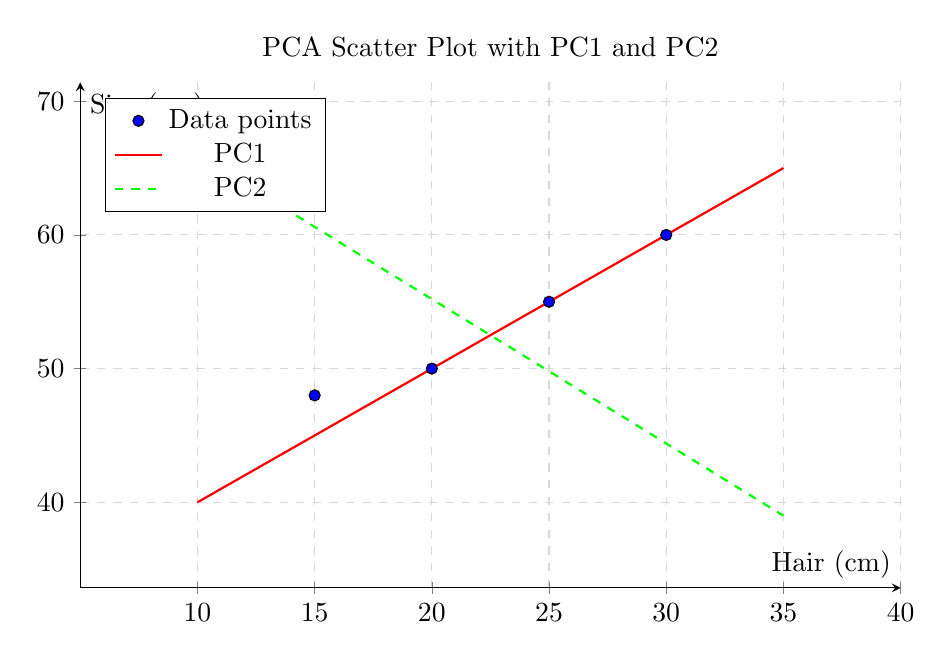
\begin{tikzpicture}
    \begin{axis}[
        width=12cm, 
        height=8cm,
        xlabel={Hair (cm)},
        ylabel={Size (cm)},
        axis lines=middle,
        grid=both,
        grid style={dashed, gray!30},
        enlargelimits=0.2,
        title={PCA Scatter Plot with PC1 and PC2},
        legend pos=north west
    ]

    % Data points (Hair, Size)
    \addplot[
        only marks,
        mark=*,
        mark options={fill=blue}
    ] coordinates {
        (20,50)
        (25,55)
        (15,48)
        (30,60)
    };

    % PC1 line (example direction)
    \addplot[
        color=red,
        thick
    ] coordinates {
        (10,40)
        (35,65)
    };

    % PC2 line (perpendicular)
    \addplot[
        color=green,
        thick,
        dashed
    ] coordinates {
        (10,66)
        (35,39)
    };

    \legend{Data points, PC1, PC2}

    \end{axis}
    \end{tikzpicture}
    \caption{PCA graph showing data points and the first two principal components (PC1 and PC2). The variables are hair and size- The PCA graph It shows, a visualization of how two data dimensions ("Hair" and "Size") can be represented in a new, transformed coordinate system that highlights the primary directions of variance- Blue= hair and size, red= longest axis and green= direction of maximum variance}
    
\end{figure}


\end{document}


